% \documentclass[]{template}    
% \begin{document}
\xjsection{绪论} 
\subsection{研究背景}
在2014年前后,Liu 等学者提出了一个新的社交网络模型:$\mathrm{EBSN}$\upcite{EBSN_linking}(图\ref{f-ebsn}),在这篇论文中,Liu 等把 $\mathrm{EBSN}$分为线上和线下两部分,人们可以线上交流,但也可以通过参与线下活动的方式线下交流。这种新型的社交网络结构有很多独有的性质,比如在事件的参与人数,组的规模及其他层面上的长尾分布,以及较之于其他传统线上社交网络上的更为强烈的局部相关性等。

由于以上原因,越来越多的学者开始关注该领域,并大致分出了几个方向:事件推荐,事件安排和其他。事件推荐更多的是从事件参与者的角度去考虑的,从事件参与者的兴趣标签出发,使用协同过滤,多标签聚类,随机游走或者其他的一些算法,来最大化某一个目标函数。由于网络规模等一些原因,获得全局最优一般是不现实的,因此相关的论文更多的是采用某些近似算法,来达到局部最优\upcite{EBSN_event_reco,EBSN_on_social}。事件安排的目的则是通过合理的安排每个事件的参与人员,在确保事件符合事件参与者的兴趣的同时,保证每个事件都符合组织者的预期:例如有足够的人参加。较之与事件推荐的不同,是事件安排同时要考虑两方面的因素,限制条件更多,例如活动参与人的限制,活动举办时间的限制和地点的限制,所以如何平衡好这方面的矛盾是解决这类问题的关键之一\upcite{EBSN_conflict-aware_2016,EBSN_feedback-aware_2017,EBSN_conflict-aware_2015}。同样,想在这类问题上获得全局最优解也是很困难的,因此通过近似算法来得到局部最优解也是普遍的选择。

\begin{figure}[htp]
    \centering
    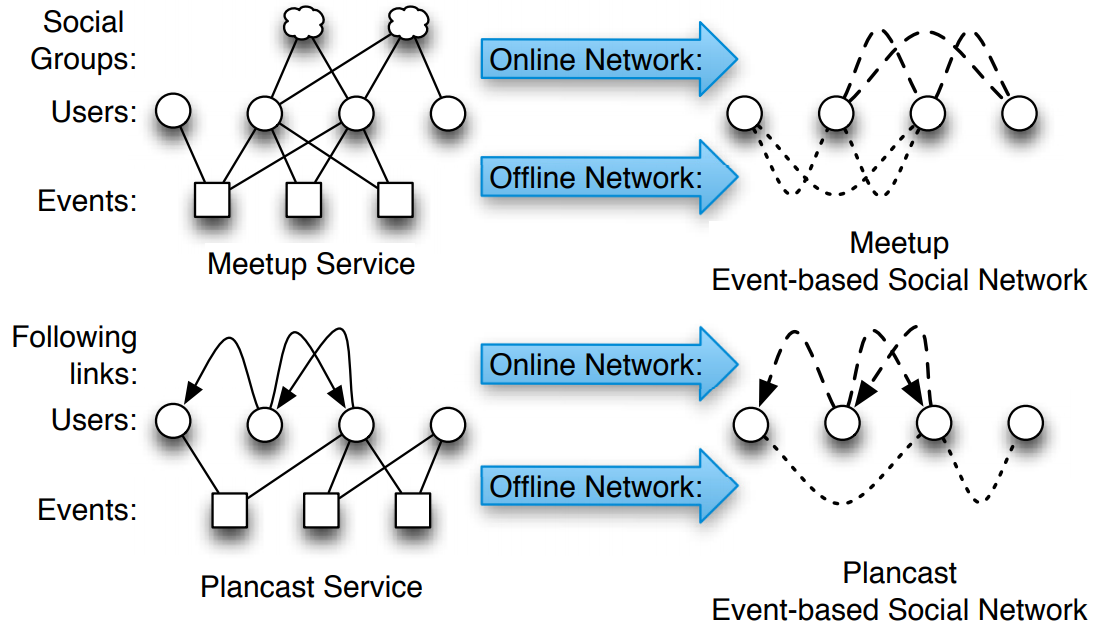
\includegraphics[width=10.4cm]{EBSN.png}
    \caption{一个典型EBSN的示例}
    \label{f-ebsn}
\end{figure}

除了以上两个方向,近年来关于EBSN的其他方向的研究也渐渐兴起。其中比较有趣的话题是通过研究$\mathrm{EBSN}$中人们如何选择和参与事件来帮助解释人群行为\upcite{EBSN_understanding},以及研究话题模型在$\mathrm{EBSN}$中的传播方式。在论文\upcite{EBSN_can_i}中,由于普遍来说一个兴趣小组的三月存活率不到百分之30,因此作者通过研究组的创办者,组成员数量的增长速度以及其他因素,来预测最终该组是否能够存活。在论文\upcite{EBSN_who_will}中,作者把角度放在了预测事件的参与人员情况上。由于人们在选择事件时会有模式可寻,因此通过学习历史数据可以预测出哪些人会有可能对一个事件感兴趣。

在$\mathrm{EBSN}$中,事件的一个属性,事件描述(\textit{event description}),提供了相当重要的信息,例如衡量事件间的相似度,和衡量与成员的契合程度。而毫无疑问,事件描述对事件结果也有很大影响。特别是在其他因素被限制的情况下(时间,地点等),事件描述给了事件举办者最大的自由度来使他的事件在其他同类事件中脱颖而出,继而能吸引更多的人来参加他举办的事件。但是如何衡量事件描述则是很困难的事情,因为评价事件描述的好坏是件相当主观的事情。这也为如何利用好事件描述里包含的信息带来了困难。而直接去定量的研究事件描述对事件结果的影响的论文更是少之又少。但这又是十分值得去研究的,本文便做了这样的尝试。

\subsection{国内外研究现状}
本文的工作和EBSN中的事件推荐和自然语言处理中的文本生成有着紧密联系。所以本节将首先介绍EBSN中关于事件推荐的相关工作,接着会介绍事件描述在事件推荐中的应用情况。最后由于本文研究了如何自动生成足够真实的事件描述,所以我们会介绍文本生成目前的研究现状。
\subsubsection{EBSN中事件推荐的相关工作}
在\upcite{EBSN_event_reco}中,Yijun等人使用图理论研究了如何在EBSN中向事件的潜在参与人群推荐合适的事件。他们首先根据EBSN的网络结构构建了一个异构网络,然后在该网络上使用反向随机游走算法构建用户——事件推荐网络,并在此基础上构建推荐列表。在\upcite{EBSN_conflict-aware_2016}中,Jieying等人率先将冲突事件的限制考虑进来,他们首先证明了在考虑冲突事件下获得事件安排的全局最优解是NP难的问题,随后他们提出了两种近似算法来获得较优解。在\upcite{EBSN_feedback-aware_2017}中,Jieying等人将事件安排的反馈考虑进推荐算法中,通过被推荐人的RSVP结果,动态调整事件的推荐权重。

\subsubsection{事件描述在事件推荐中的应用}
事件描述作为事件的一个属性,在事件推荐中起到非常重要的作用。然而,到目前为止,几乎所有的论文中,事件描述都只被用来衡量事件间的相似度,以及事件与用户兴趣的契合度。比如在\upcite{EBSN_who_will}中,事件描述被用来计算事件间的相似度,这样便可以根据用户参与事件的历史数据,来给他推荐相似的事件。而在\upcite{gu_context_2016}中,Gu等人使用TF-IDF算法来处理事件描述,并用其计算事件间的相似度。通过以上论文,我们可以看出,目前关于事件描述的运用还非常局限。而在\upcite{event_organization_101}中,Shuo等人提出用Vader对事件描述进行情感分析,并使用Jaccard相似度来衡量事件的新奇性。这也是据本文作者所知唯一一篇直接使用事件描述来对事件进行评价的论文。

\subsubsection{文本生成研究现状}
在自然语言处理中,目前运用最广泛的模型之一是Mikolov等人提出的RNNLM\upcite{mikolov_rnnlm_2011}。而在文本生成领域,也有很多运用和改进RNNLM的例子。在\upcite{Chinese_Poetry}中,Xingxing等人运用一个RNN来生成中国诗。他们通过训练RNN学习单个字的表示,来使生成器学会生成在内容和平仄上都符合规范的古诗。在\upcite{kim_character-aware_2015}中,Kim等人对RNNLM做了改进,他们使用单个字符而非单个单词作为输入,在RNNLM前加入了卷积层和highway层,使得模型从字符的角度,而非单词的角度学会了如何表达自然语言。实验证明他们的改进模型能大大减少参数数量,并且在学习富词法语言中,表现优于传统的以词为最小单位的语言模型。

为了让RNNLM在生成文本时除了依赖当前状态,还依赖某个全局表达,以达成生成符合期望的文本的目的,人们提出了seq2seq模型,这样在生成文本的过程就成了编码-解码的过程。编码器首先将某段文本表示成一个隐向量,再通过解码器解码,以次达到对输出文本的控制效果。seq2seq模型被广泛运用于机器翻译和问答系统的设计中。在编码器的选择上,也有许多不同方案。在\upcite{bowman_generating_2015}中,Bowman等人率先将变分自编码器引入文本生成中,他们利用变分自编码器通过采样得到编码的特性,确保了隐编码能够服从特定分布,从而保证了编码的连续性和局部相关性。而在\upcite{noauthor_sequence_nodate}中,Muller等人也利用了变分自编码器编码空间连续的特性,通过一个对特定文本的编码进行梯度上升操作,来最大化某个目标函数,从而达到改进某段文本的目的。

为了使生成文本表现的更像真实文本,生成对抗网络也被引入到文本生成领域中。在\upcite{yu_seqgan:_2016}中,yu等人设计了SeqGAN,一个使用RNNLM作为生成模型,以及带卷积层的神经网络作为判别模型的生成对抗网络,来训练生成模型生成和真实文本接近的文本序列。而在\upcite{lin_adversarial_2017}中,Lin等人也采用了类似的结构,通过训练生成模型生成评分胜过真实训练数据的文本,来使其可以生成足够真实的文本序列。

\subsection{主要工作}
本文主要工作如下:1)本文使用了不同的分类算法,比较了包含和不包含事件描述的情况下,对预测事件结果的准确率的影响,并使用固定系数来衡量事件描述对模型解释性的提升,证明了事件描述对事件举办结果的重要性。2)本文设计了带GRU的神经网络,和另外两个传统的文本处理模型(线性回归,卷积神经网络)共同处理事件描述,并用其来预测事件参与人数和事件结果。实验证明本文提出的模型能够将预测事件参与人数与真实人数的均方误差控制在0.2左右,大大超过了基准模型。3)本文设计了基于差分自编码器和生成对抗网络的文本生成模型,来训练模型生成接近真实事件描述的文本序列。
\subsection{论文组织结构}
本文包括了如下六章,每章的组织如下:

第一章简要概述了当前问题的研究背景和EBSN网络中关于事件结果预测和文本生成的研究现状,接着简单介绍了本文的主要工作,并在最后说明了本文的组织结构。

第二章主要介绍研究问题的相关工作,先介绍了EBSN中事件描述,事件参与度和事件结果等名词,以及在目前有关EBSN的研究工作中,对事件描述的运用。最后则简单描述了目前文本生成方面的进展。 

第三章会先简单介绍本文研究对象,并定量的研究事件描述对事件参与人数的影响。本文首先给出了事件结果的定义,然后提出了事件相似度并以此为根据对事件结果进行标注,并比较了事件描述属性在多种分类算法下对预测事件结果的影响。最后通过事件描述对随机效应的确定系数的影响,本文证明了事件描述在事件属性中的重要性。

第四章介绍本文在使用事件描述预测参与人数方面的工作。本文通过设计了带卷积层的神经网络和带GRU的神经网络用来处理文本属性,并使用实验证明相较于第三章使用的文本处理方式,带GRU 的神经网络能够将事件结果预测的准确率提升2个百分点。

第五章介绍事件描述生成模型。本文使用了变分自编码器作为生成模型,使用第四章提出的带GRU的神经网络作为判别模型,来训练其生成接近真实事件描述的文本序列。实验证明经过训练后,本文提出的事件描述生成模型可以产生与真实文本足够相似的事件描述。

第六章是总结和展望,本文会总结本文工作,并讨论其未来的改进的空间。


% \end{document} 

